\subsection{Regularization}

Among all unbiased solutions $(X^TX)^{-1}X^TY$ is the solution that has the smallest variance $\Rightarrow$ minimizes gen. Error

One can set the $\omega$ of higher order features manually to zero ($\leftrightarrow$ choose a less complex model) or

\textbf{Ridge Regression} $\underset{\omega}{min}||Y-X\omega||^2 + \lambda||\omega||^2$

Always allows for closed solution and lets LS converge faster (EVs of Hessian $X^TX$ change)

Equivalent to performing Bayesianism approach with $p(\omega) = \mathcal{N}(\omega|0,\boldsymbol{\Lambda}^{-1})$ or linearly $p(\omega) = \mathcal{N}(\omega|0,1)$

\textbf{Lasso Regression} $\underset{\omega}{min}||Y-X\omega||^2 + \lambda|\omega|$ 

Convex loss  but no closed form solution (not differentiable)

Bayes. w/ Laplacian prior:  $p(\omega_i) = \frac{\lambda}{4\sigma^2}exp(-|\omega_i|\frac{\lambda}{w\sigma^2})$

$\omega_{\text{high}} \rightarrow 0 \Rightarrow$ sparse, $\lambda_{opt}$ through CV.

% \begin{center}
%     \resizebox{0.6\linewidth}{!}{
%     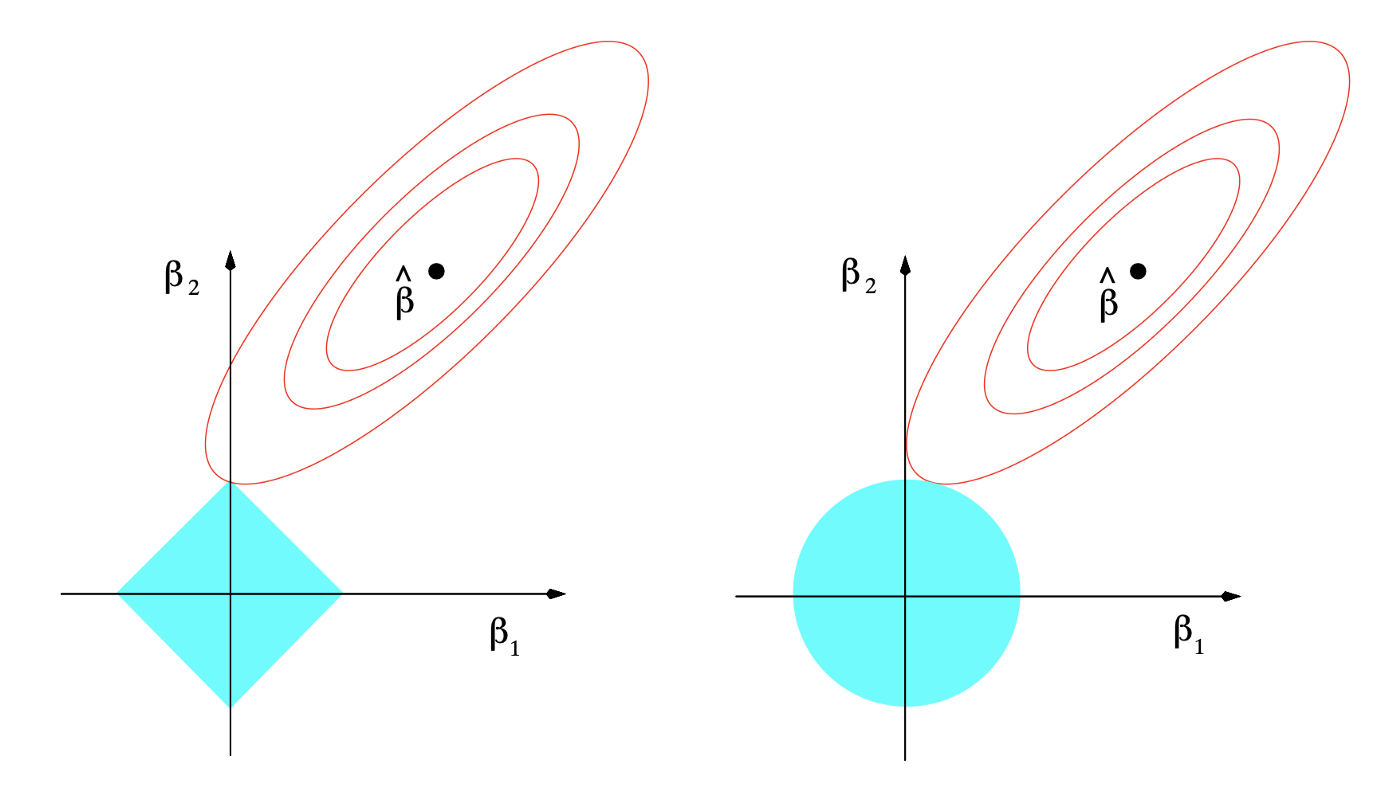
\includegraphics{images/lasso_vs_ridge.png}
%     }
% \end{center}
% Left: Lasso, Right: Ridge


